\section{Results}

After training, the model was evaluated using the testing set,
achieving an overall accuracy of approximately 88%. The model's
performance was further analyzed using metrics such as recall and
precision. The recall score, which measures the model's ability to
correctly identify true positives, was found to be 0.86. The
precision score, which measures the model's ability to avoid false
positives, was found to be 0.89. These results indicate that the
model has a high degree of accuracy in detecting both real and fake
images.
Below are the confusion matrix and graphs illustrating the training
and validation accuracy over epochs. These visualizations provide a
comprehensive overview of the model's performance and can be
used to further analyze its strengths and weaknesses.

\begin{figure}[h]
    \centering
    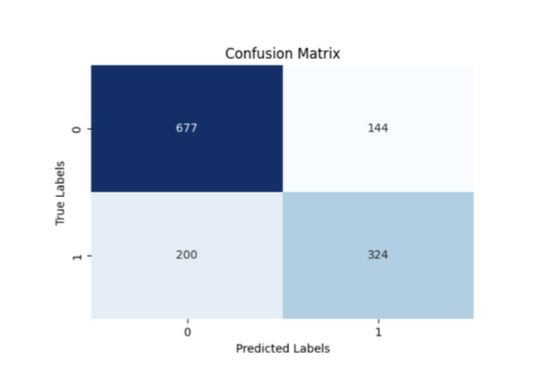
\includegraphics[width=1\textwidth]{figures/confusion_matrix.png}
    \caption{Confusion Matrix}
    \label{fig:enter-label}
\end{figure}


\begin{figure}[h]
    \centering
    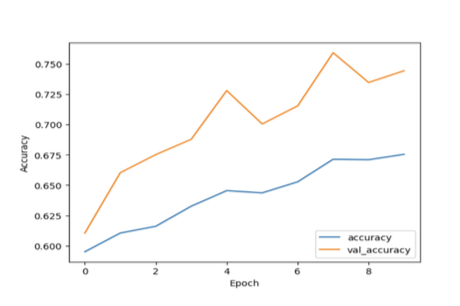
\includegraphics[width=1\textwidth]{figures/accuracy_epoch.png}
    \caption{Accuracy v/s Epoch}
    \label{fig:enter-label}
\end{figure}


























